%\documentclass[a4,semhelv,landscape]{seminar}
\documentclass[landscape]{slides}
%\documentclass[pdf, default, slideBW, nocolorBG]{prosper}
\usepackage[left=0.2cm,top=0.2cm,right=0.2cm,bottom=0.2cm,nohead,nofoot]{geometry}
%\def\everyslide{\sffamily}
%\usepackage{fullpage}
\usepackage{graphicx}
\usepackage[usenames]{color}
%\usepackage{color}
\usepackage{verbatim}
\usepackage{nopageno}
\usepackage{setspace}
%\usepackage{times}
% define some nice colors
\definecolor{myred}{rgb}{0.6,0,0}
\definecolor{myblue}{rgb}{0,0.2,0.4}
\definecolor{mygreen}{rgb}{0,0.5,0.0}
\definecolor{mypurple}{cmyk}{0.5,1.0,0.0,0.0}
\definecolor{myorange}{cmyk}{0.0,0.75,1.0,0.0}
%\color{myblue}

\begin{document}
%%%%%%%%%%%%%%%%%%%%%%%%%%%%%%%%%%%%%%%%%%%%%%%%%%%%%%%%%%%%%%%%%%%%
%Slide 0 - title
\begin{slide}
\begin{center}
\large{\textbf{Reference-based viral sequence annotation using VADR}}

\normalsize

Eric Nawrocki \\

\medskip

\medskip

\medskip

\medskip

\medskip

\small
\begin{tabular}{c}
%Alejandro Sch\"{a}ffer's group \\
%\\
National Center for Biotechnology Information\\
National Institutes of Health\\
\\
\end{tabular}

\vspace{0.1in}


\includegraphics[width=2.5in]{figs/ncbi-logo}

\end{center}
\end{slide}
%%%%%%%%%%%%%%%%%%%%%%%%%%%%%%%%%%%%%%%%%%%%%%%%%%%%%%%%%%%%%%%%%%%%%%
\begin{slide}
\begin{center}
\textbf{GenBank has a lot of sequences}
\end{center}

\vfill
\end{slide}
%%%%%%%%%%%%%%%%%%%%%%%%%%%%%%%%%%%%%%%%%%%%%%%%%%%%%%%%%%%%%%%%%%%%%%
\begin{slide}
\begin{center}
\textbf{Sequence submissions are handled by expert NCBI indexers}
\end{center}

\small
\begin{itemize}
\item Indexers check submissions for quality
\item Many submissions are of \emph{marker genes}, used to
  characterize environments (microbiome, soil), which are
  automatically analyzed by BLAST or specialized tools.
%\item Submissions with zero errors automatically enter database
%  (``foosh'')
%\item Submissions with errors can be corrected by submitter or are manually reviewed by an indexer
\end{itemize}

\medskip

\begin{center}
\begin{tabular}{l||r|r||r||l}
                                 &    2018  & total     &         &           \\
 marker gene/                    &  GenBank & GenBank   &  TLS\footnote{TLS: Targeted Locus Study, currently only 16S submissions with $>=$ 2500 seqs}      & analysis  \\
 sequence type                   &  \# seqs & \# seqs   & \# seqs & tool \\ \hline
& & & \\                    
%\textcolor{red}{16S rRNA}        & \textcolor{red}{333,121}  & \textcolor{red}{8,015,297} & \textcolor{red}{18,262,402} & \textcolor{red}{BLAST}\footnote{TLS submissions now processed with Ribosensor} \\
%16S rRNA                        & 333,121  & 8,015,297 & 18,262,402 & BLAST$^{*}$ \\
16S rRNA                        & 333,121  & 8,015,297 & 18,262,402 & BLAST \\
& & & \\                    
 23S rRNA                        & 74,287  &   275,014  & 2,140      & BLAST \\
& & & \\
 ITS1                            & 27,279  &   359,380  & 13,294     & BLAST \\
& & & \\                    
 ITS2                            & 24,144  &   184,515  &      0     & BLAST \\
& & & \\                    
 ITS1+ITS2                       & 26,734  &   445,721  & 25,725     & BLAST \\
& & & \\                    
 Influenza A                     & 74,868  &   665,464  &      0     & FLAN \\
\end{tabular}
\end{center}
\vfill
\tiny \flushleft{$\dagger$ TLS: Targeted Locus Study, currently only 16S submissions with $>=$ 2500 seqs, handled by Anji Johnston}
%\tiny \flushleft{$\ddagger$ TLS submissions now processed with ribosensor}
\end{slide}
%%%%%%%%%%%%%%%%%%%%%%%%%%%%%%%%%%%%%%%%%%%%%%%%%%%%%%%%%%%%%%%%%%%%%%
\begin{slide}
\begin{center}
\textbf{NCBI GenBank Indexers have large backlogs}

\begin{itemize}
\item Indexer: evaluate a sequence submission and associated metadata
  and either:
  \begin{itemize} 
    \item accept for deposition to GenBank
    \item communicate with submitter to resolve \emph{problems}
  \end{itemize}

\item \textbf{Goal: automate as much as possible}
  \begin{itemize}
  \item Evaluate with an annotation tool and submissions with zero
    errors automatically enter database
    (``foosh'')
  \end{itemize}
  \item Foosh pipelines exist for 16S, 23S, ITS (BLAST-based) and
    Influenza (FLAN)
\end{itemize}

\vfill
\end{center}
\end{slide}
%%%%%%%%%%%%%%%%%%%%%%%%%%%%%%%%%%%%%%%%%%%%%%%%%%%%%%%%%%%%%%%%%%%%%%
\begin{slide}
\begin{center}

\textbf{Viruses with highest number of sequences in GenBank\footnote{as of October, 2019.}}

\tiny
\begin{tabular}{lrl}
species                   &       \#seqs & family           \\ \hline
%                                                              % taxids
& & \\
HIV-1                     &      850,115 & \emph{Retroviridae}     \\ % 11676
& & \\
Influenza A virus         &      684,026 & \emph{Orthomyxoviridae} \\ % 11320
& & \\
Hepacivirus C             &      244,533 & \emph{Flaviviridae}     \\ % 11103
& & \\
Hepatitis B virus         &      114,306 & \emph{Hepadnaviridae}   \\ % 10407
& & \\
Influenza B virus         &      100,373 & \emph{Orthomyxoviridae} \\ % 11520
& & \\
Rotavirus A               &       73,375 & \emph{Reoviridae}       \\ % 28875
& & \\
SIV                       &       44,374 & \emph{Retroviridae}     \\ % 11723
& & \\
Norovirus (Norwalk virus) &       40,925 & \emph{Caliciviridae}    \\ % 11983
& & \\
Enterovirus A             &       31,478 & \emph{Picornaviridae}   \\ % 138948
& & \\
PRRSV                     &       29,081 & \emph{Arteriviridae}    \\ % 28344
& & \\
Dengue virus              &       28,564 & \emph{Flaviviridae}     \\ % 12637
& & \\
Human orthopneumovirus    &       24,384 & \emph{Pneumoviridae}    \\ % 11250 (RSV) 
& & \\
Enterovirus B             &       23,865 & \emph{Picornaviridae}   \\ % 138949
& & \\
Rabies lyssavirus         &       23,771 & \emph{Rhabdoviridae}    \\ % 11292
& & \\
West Nile virus           &       21,563 & \emph{Flaviviridae}     \\ % 11082
& & \\
Measles morbillivirus     &       17,233 & \emph{Paramyxoviridae}  \\ % 11234
\end{tabular}




\vfill

\end{center}
\end{slide}

%%%%%%%%%%%%%%%%%%%%%%%%%%%%%%%%%%%%%%%%%%%%%%%%%%%%%%%%%%%%%%%%%%%%%%
\begin{slide}
\begin{center}
\textbf{Viral sequences are not systematically or thoroughly annotated}
\end{center}

\small
\begin{itemize}
\item Examples of incomplete annotation: 
  \begin{itemize}
  \item Rfam families are rarely to never annotated in viral genomes
    (roughly 200 families)
  \item Less than 2\% of Norovirus sequences have mature peptide
    annotation. 
\end{itemize}
\item Systematic and complete annotation would benefit viral
  researchers and facilitate comparative analyses
\end{itemize}

\vfill
\end{slide}
%%%%%%%%%%%%%%%%%%%%%%%%%%%%%%%%%%%%%%%%%%%%%%%%%%%%%%%%%%%%%%%%%%%%%%
\begin{slide}
\begin{center}
  \item VADR (Viral Annotation DefineR) uses RefSeqs to validate and
    annotate viral sequences

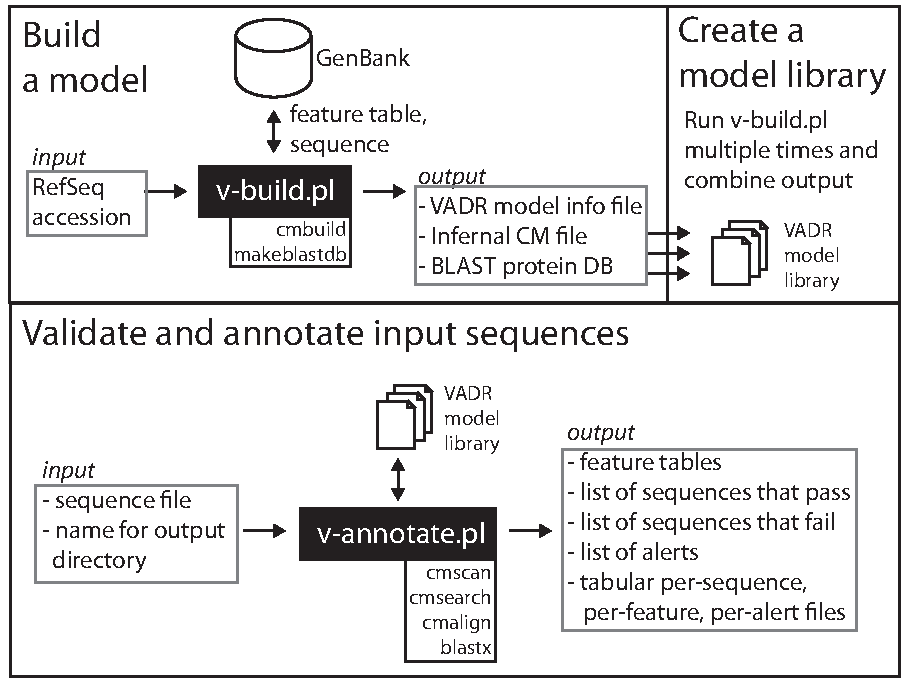
\includegraphics[width=7in]{figs/vadr}
\end{center}

\small
\begin{itemize}
  \item We chose Norovirus and Dengue virus sequences for the pilot
    project.
\end{itemize}

%\small
%\begin{itemize}
%\item Build a model (covariance model) from a RefSeq (or alignment) using \texttt{v-build.pl}
%\begin{itemize}
%  \item includes boundaries of CDS, mat\_peptide, ncRNA and other features
%\end{itemize}

%\item Incoming sequences are compared against a library of models to find
%  the best-matching model which is used to annotate the sequence using
%  \texttt{v-annotate.pl}.

%%%%%%%%%%%%%%%%%%%%%%%%%%%%%%%%%%%%%%%%%%%%%%%%%%%%%%%%%%%%%%%%%%%%%%
\begin{slide}
\begin{center}
\textbf{VADR-based sequence validation: unexpected characteristics are identified and reported 
  as \emph{alerts}}
\end{center}

\scriptsize
\begin{itemize}
\item Examples of alerts: early stop codon, dissimilar region
\item Some alerts are \emph{fatal}
\item Sequences with 1 or more fatal alerts \emph{fail}
\item Sequences with 0 fatal alerts \emph{pass} and are cleared for
  entry into GenBank (foosh).
\end{itemize}

\vfill
\end{slide}
%%%%%%%%%%%%%%%%%%%%%%%%%%%%%%%%%%%%%%%%%%%%%%%%%%%%%%%%%%%%%%%%%%%%%%
\begin{slide}
\begin{center}

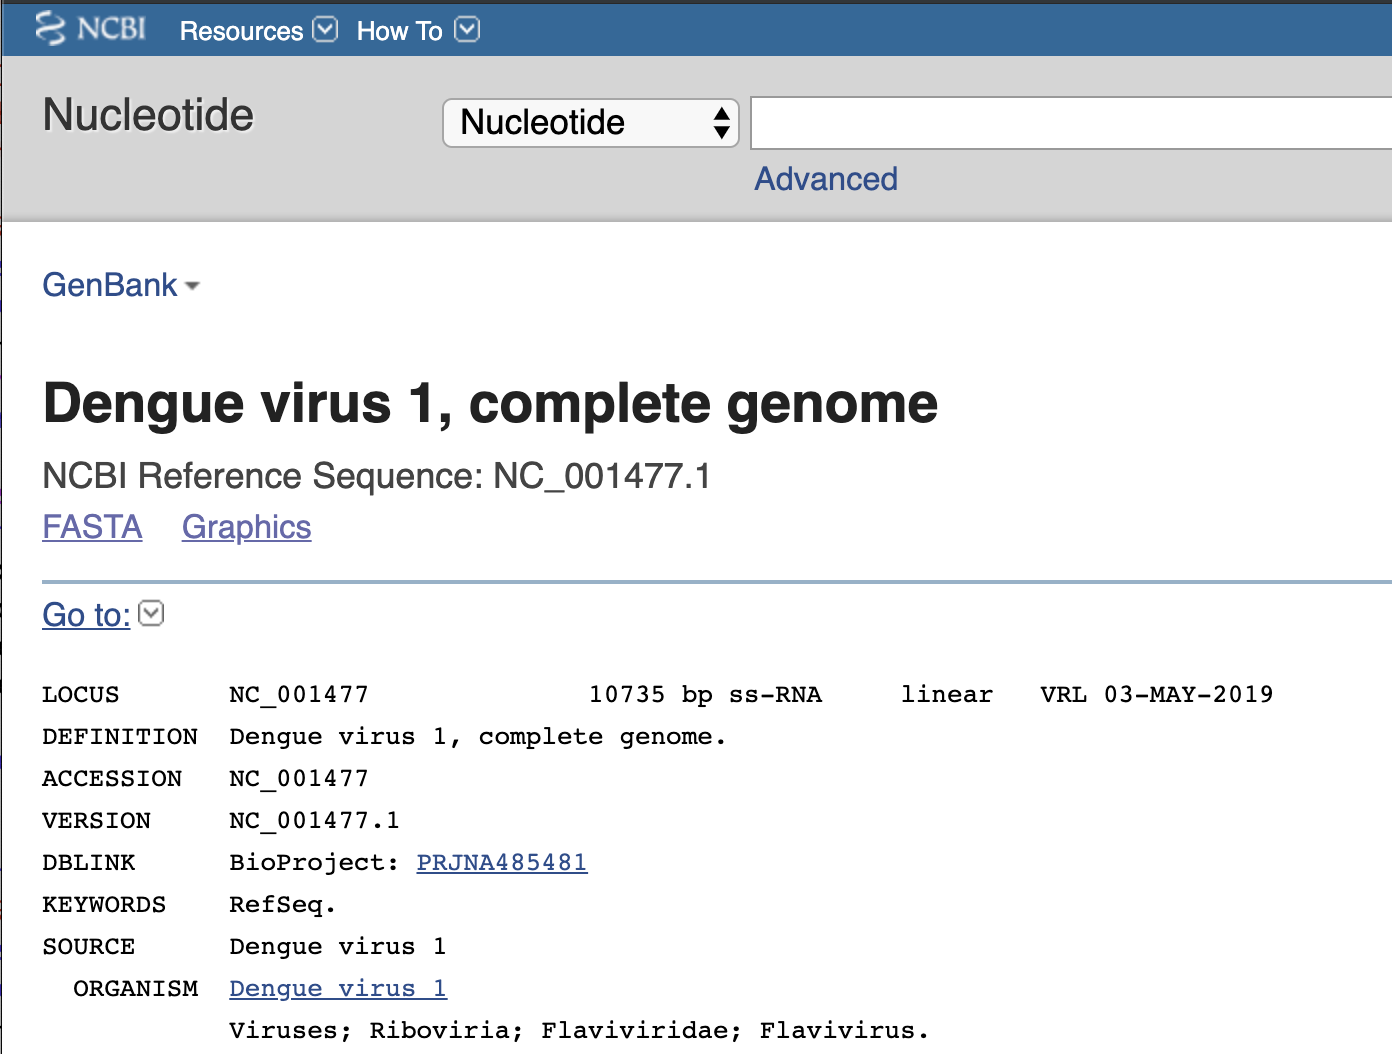
\includegraphics[width=6in]{figs/ss-001477-top}
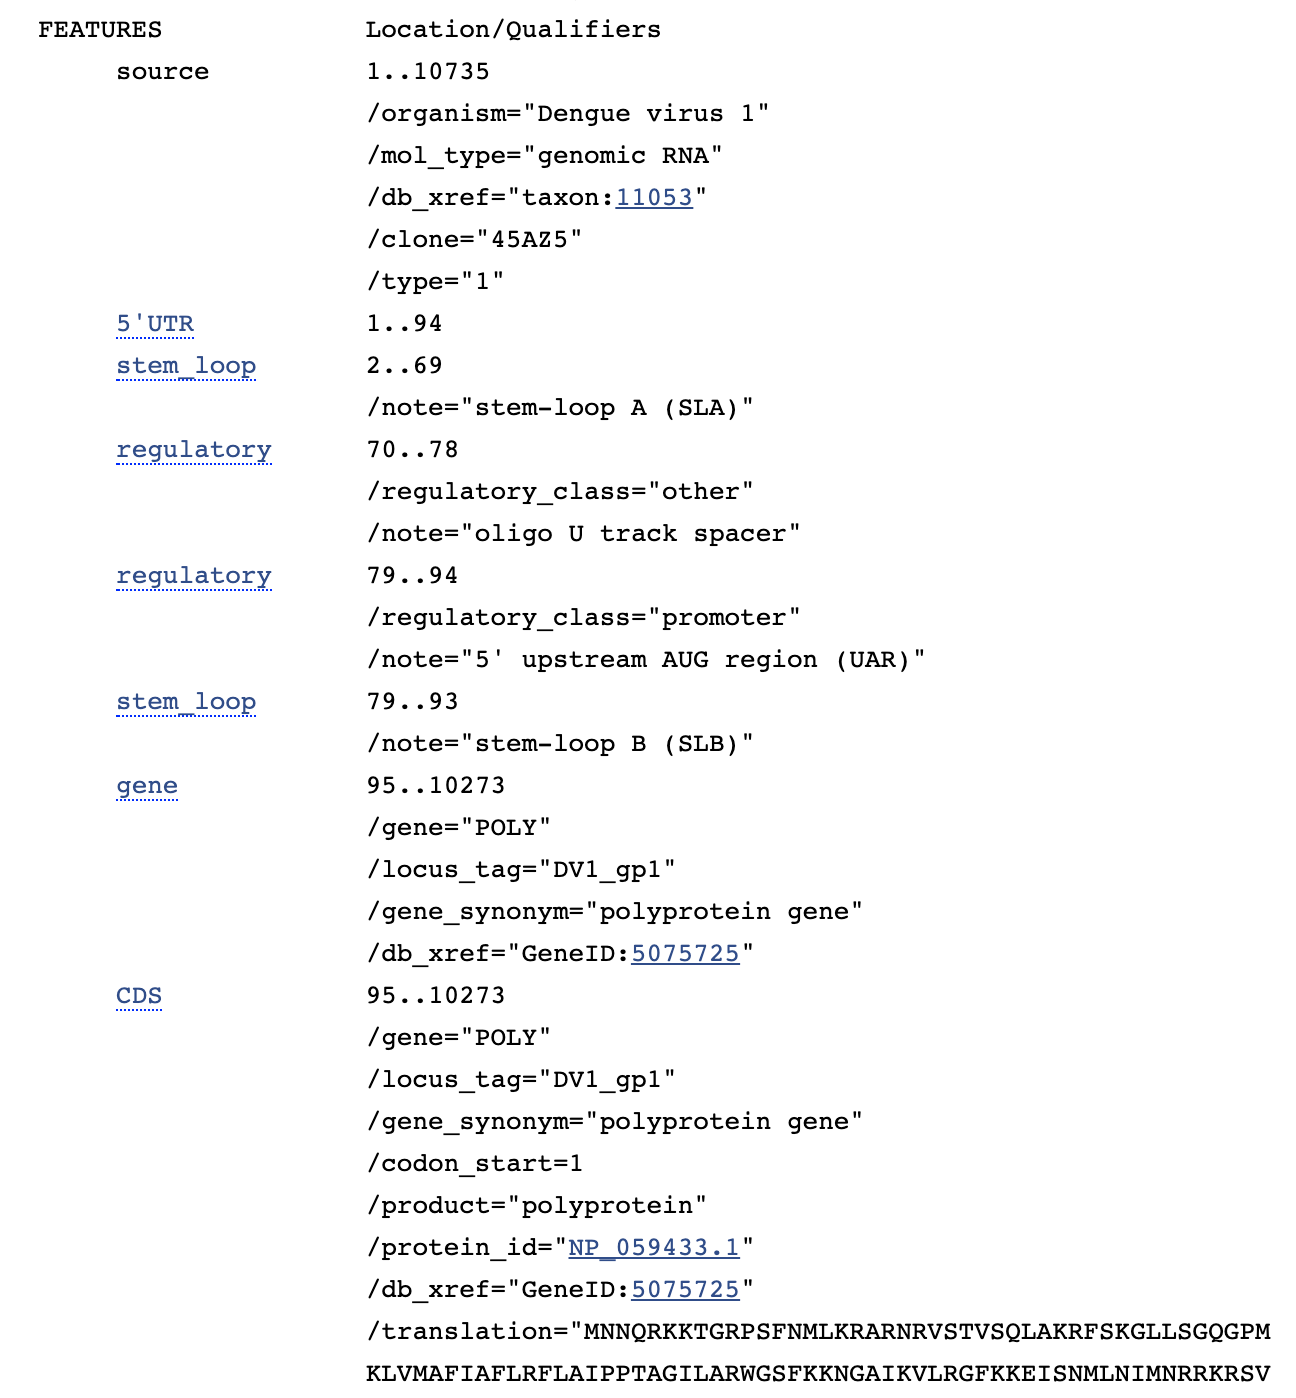
\includegraphics[width=6in]{figs/ss-001477-mid}

\end{slide}
%%%%%%%%%%%%%%%%%%%%%%%%%%%%%%%%%%%%%%%%%%%%%%%%%%%%%%%%%%%%%%%%%%%%%%
\begin{slide}
\begin{center}

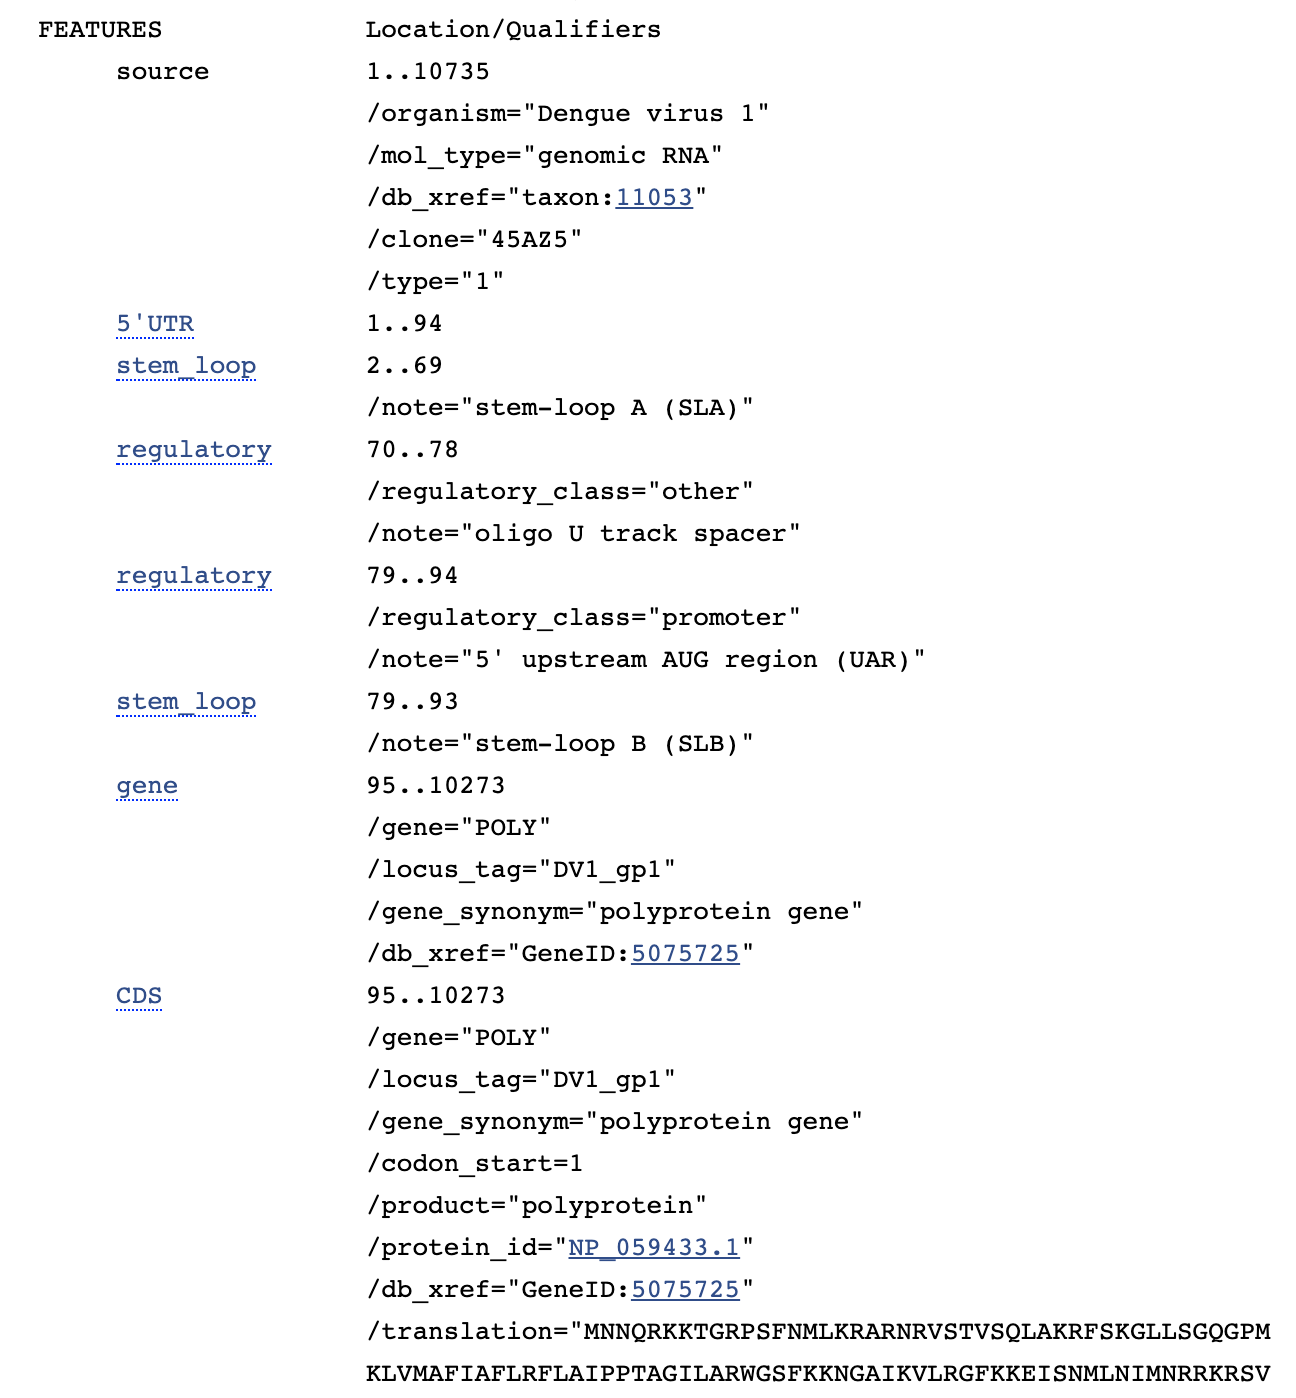
\includegraphics[width=6in]{figs/ss-001477-mid}
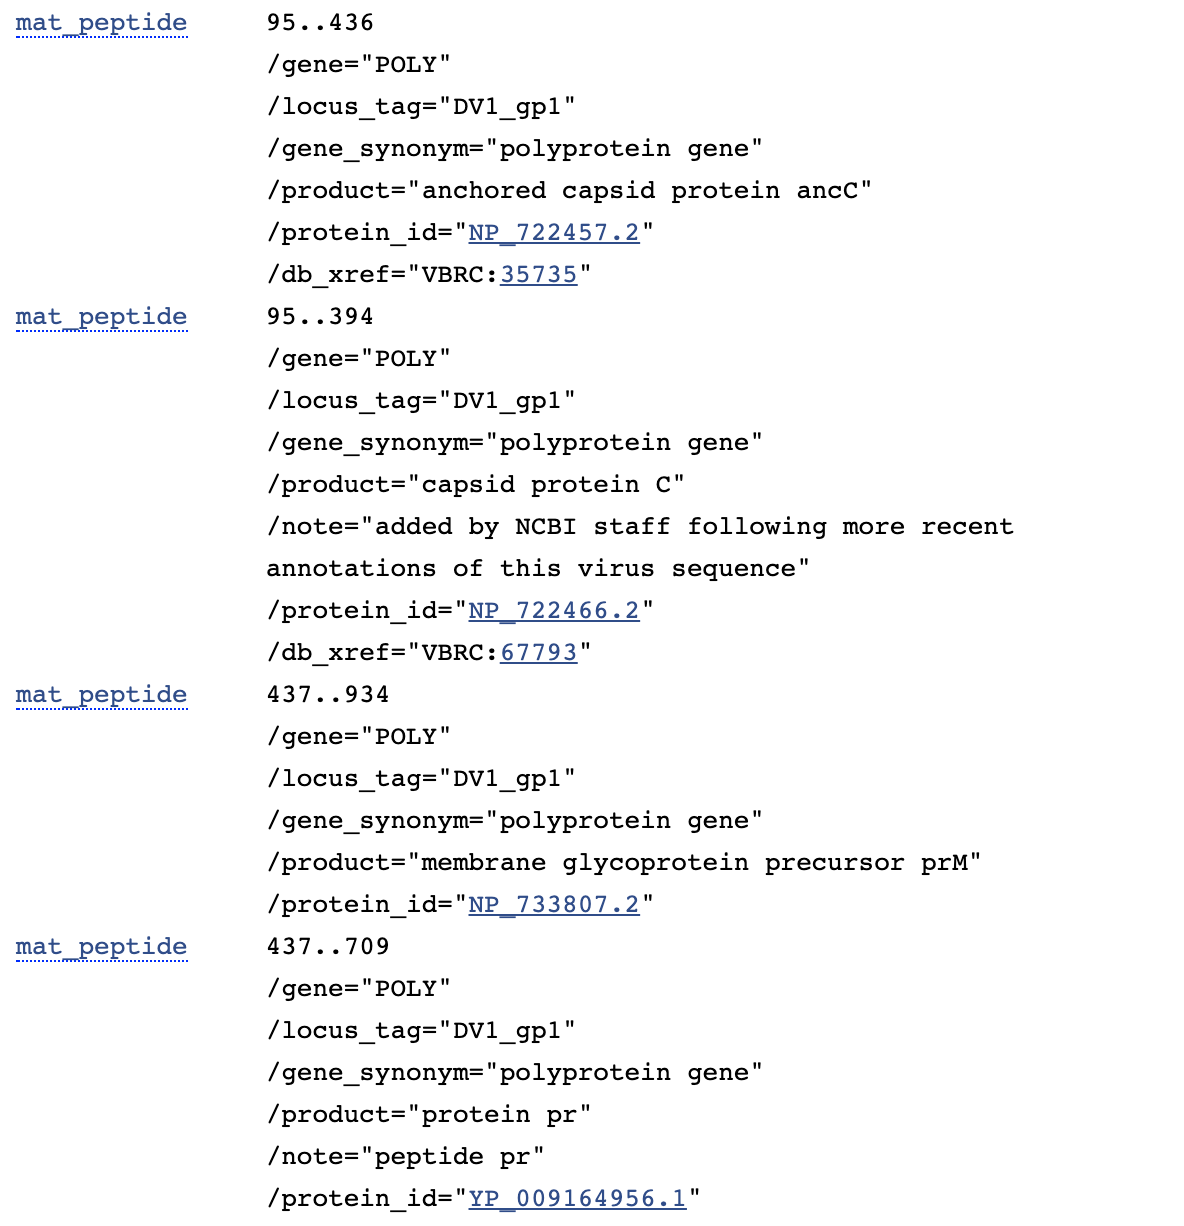
\includegraphics[width=6in]{figs/ss-001477-bot}

\end{slide}
%%%%%%%%%%%%%%%%%%%%%%%%%%%%%%%%%%%%%%%%%%%%%%%%%%%%%%%%%%%%%%%%%%%%%%
\begin{slide}
\begin{center}

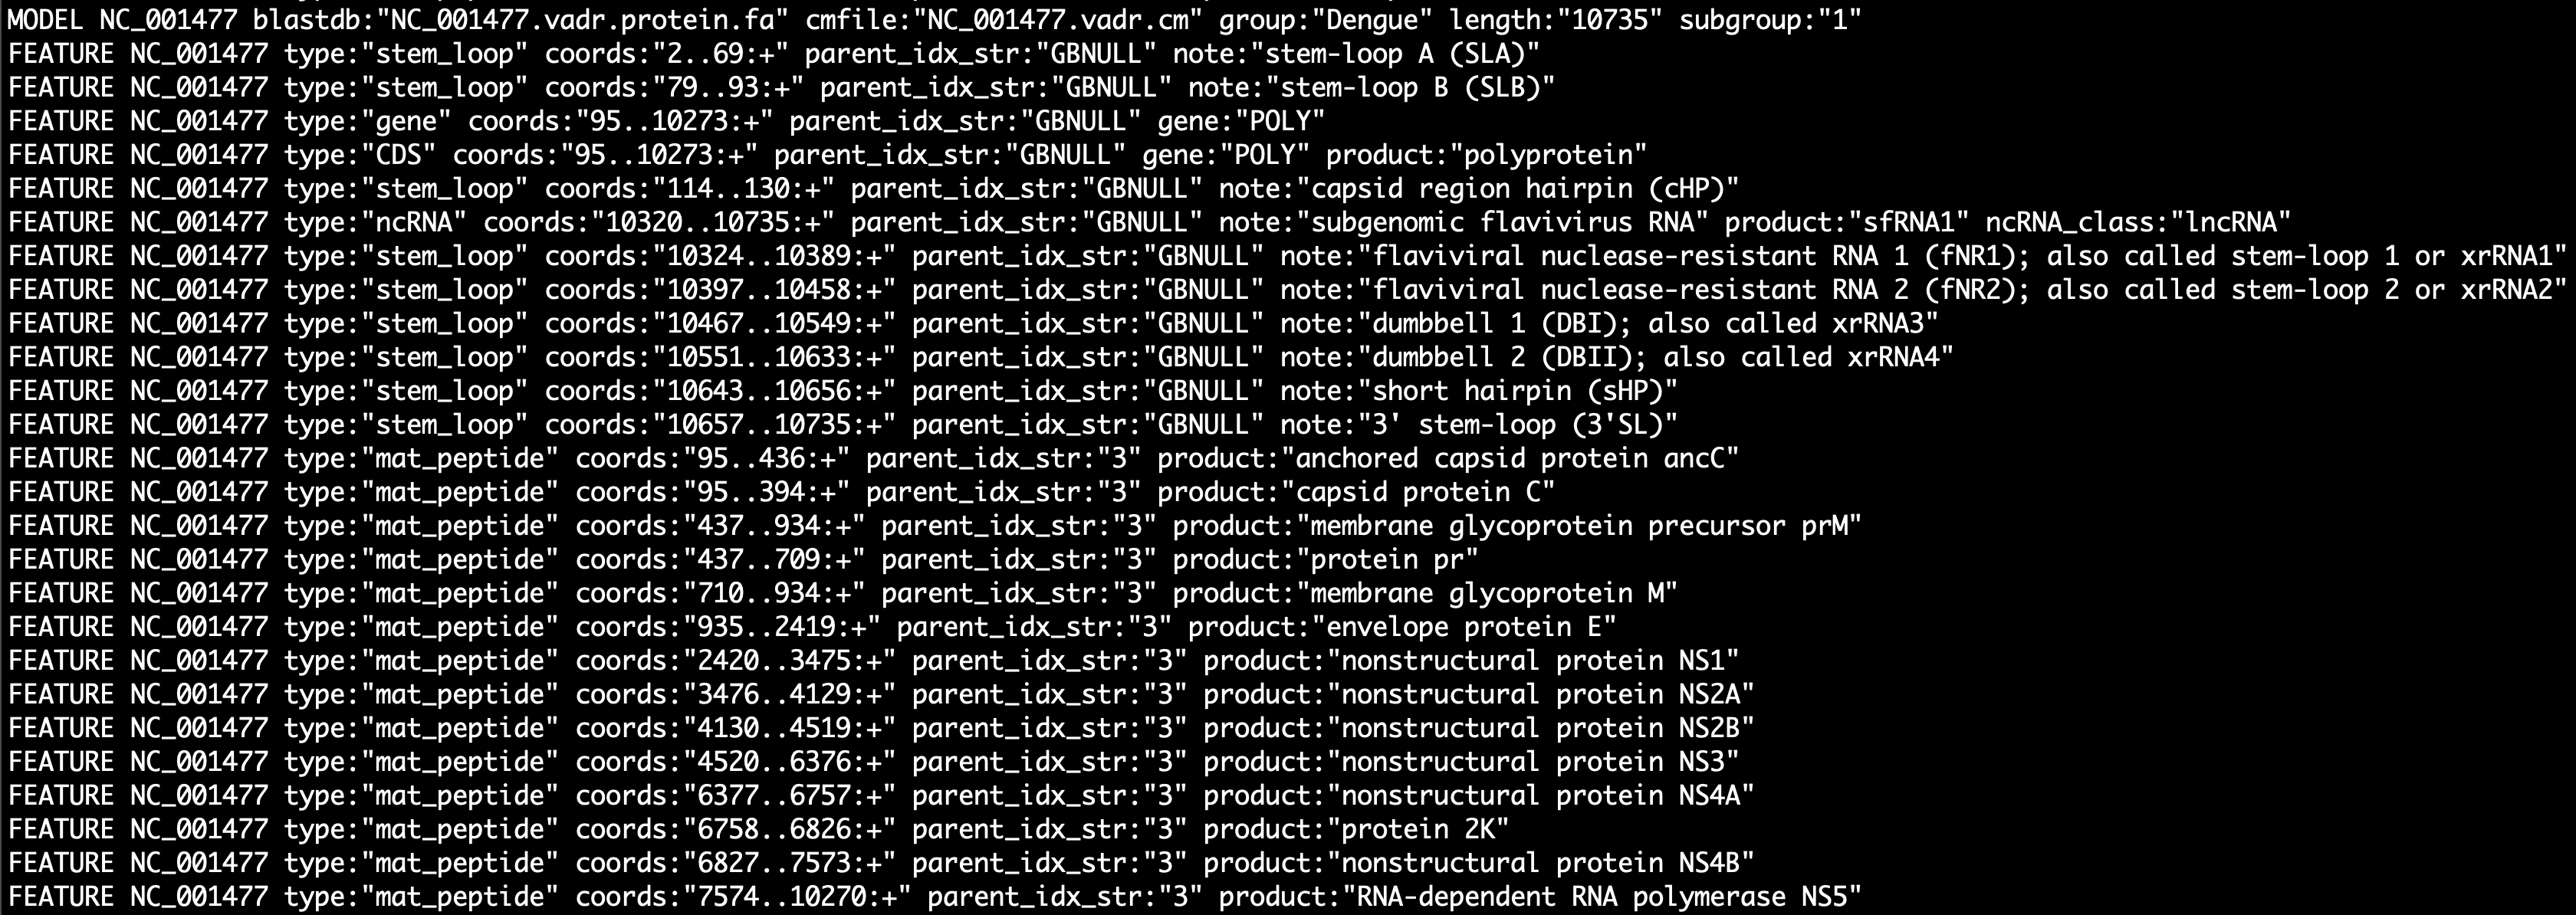
\includegraphics[width=9in]{figs/ss-001477-minfo}

\end{slide}
%%%%%%%%%%%%%%%%%%%%%%%%%%%%%%%%%%%%%%%%%%%%%%%%%%%%%%%%%%%%%%%%%%%%%%
%%%%%%%%%%%%%%%%%%%%%%%%%%%%%%%%%%%%%%%%%%%%%%%%%%%%%%%%%%%%%%%%%%%%%%
\begin{slide}
\begin{center}
\textbf{\texttt{v-annotate.pl} annotates each sequence using its
  best-matching model}

\small
\begin{description}
\item[Classification]: Each sequence is compared against all models 
  to determine its best-matching model to determine score only (no
  hit boundaries)

\item[Coverage determination]: Each sequence is compared against
  its best matching model again to obtain hit boundaries

\item[Alignment]: Each sequence is aligned to its best-matching
  model (globally with respect to sequence, locally with respect to
  the model) and feature annotation is mapped from model to sequence

\item[Protein validation]: Predicted CDS features in each sequence are
  compared against proteins from Reference model using BLASTX
\end{description}

\emph{Different types of alerts are identified and reported at each stage}

\end{center}

\vfill
\end{slide}
%%%%%%%%%%%%%%%%%%%%%%%%%%%%%%%%%%%%%%%%%%%%%%%%%%%%%%%%%%%%%%%%%%%%%%
\begin{slide}
\begin{center}

\begin{description}
\item[Classification]: Each sequence is compared against all models 
  to determine its best-matching model to determine score only (no
  hit boundaries)
\end{description}

\begin{itemize} 
\item First three stages of the HMMER3 pipeline are used to
  determine score quickly using a ``profile'' HMM of each model
  (single RefSeq).
\end{itemize}

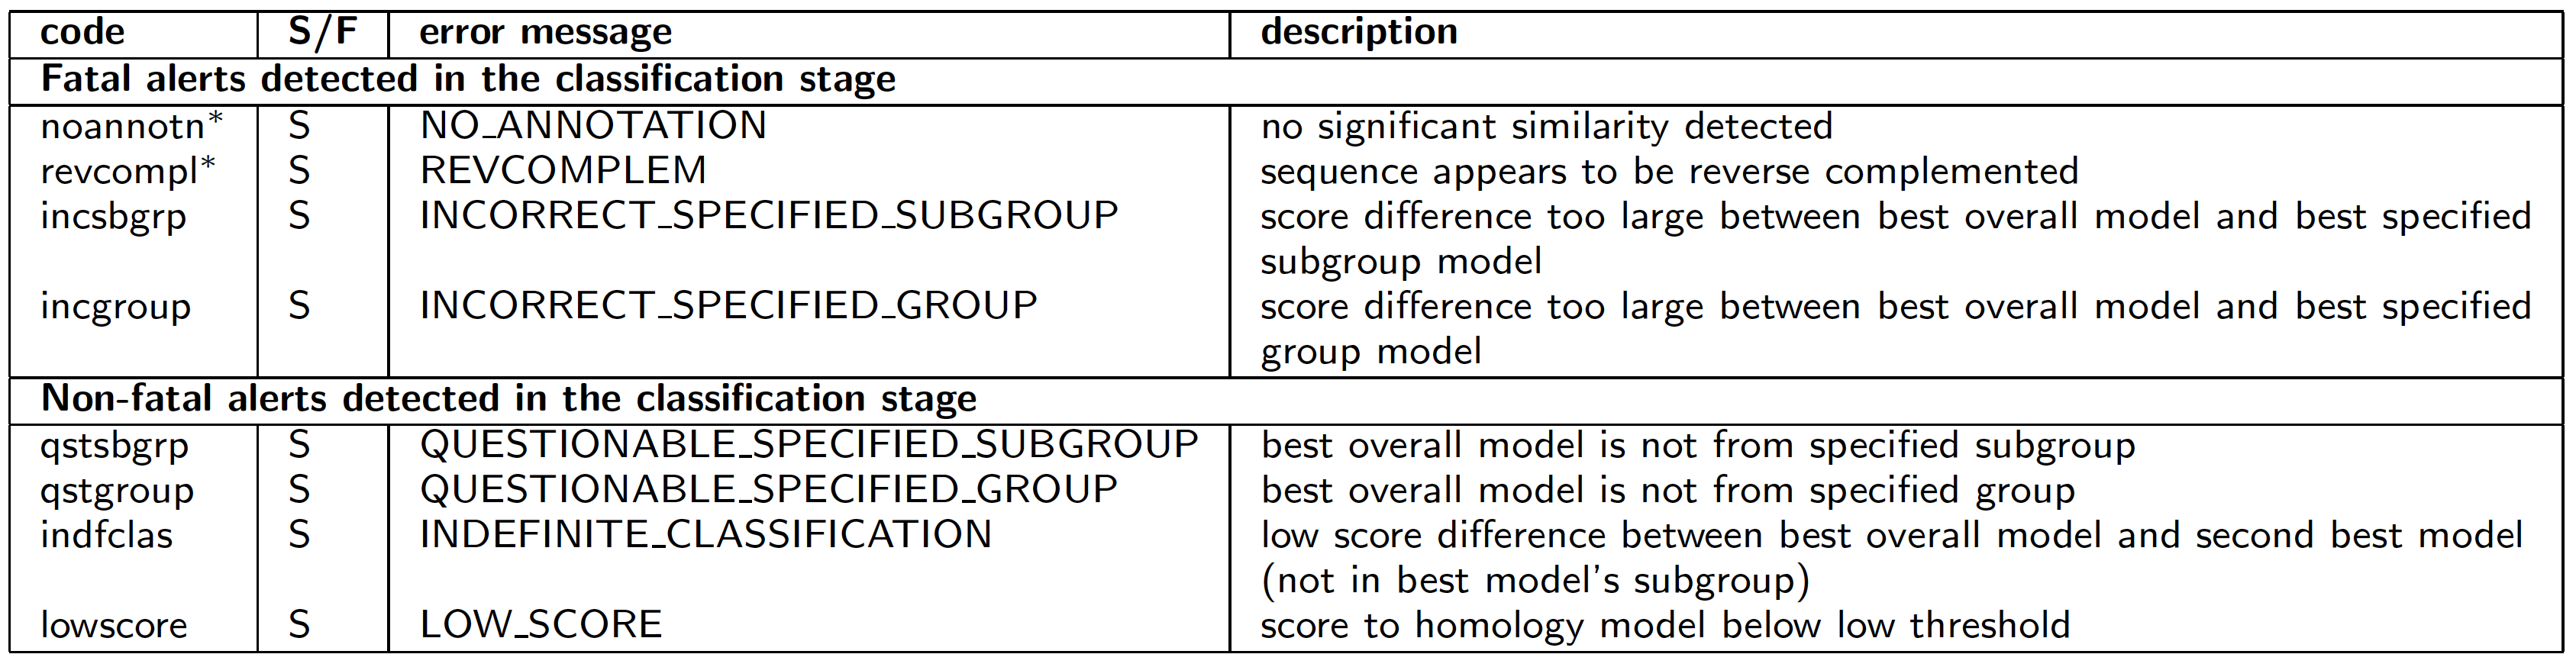
\includegraphics[width=6in]{figs/ss-class-alert-list}

\end{center}
\vfill
\end{slide}
%%%%%%%%%%%%%%%%%%%%%%%%%%%%%%%%%%%%%%%%%%%%%%%%%%%%%%%%%%%%%%%%%%%%%%
\begin{slide}
\begin{center}
\textbf{\texttt{v-annotate.pl}: coverage determination stage}
\end{center}

\begin{description}
\item[Coverage determination]: Each sequence is compared against
  its best matching model again to obtain hit boundaries
\end{description}

\begin{itemize} 
\item Full HMMER3 pipeline is used using best-matching model to 
  determine hit boundaries. Allows additional types of ``problems'' to
  be detected. 
\end{itemize}

Possible alert types:

\vfill
\end{slide}
%%%%%%%%%%%%%%%%%%%%%%%%%%%%%%%%%%%%%%%%%%%%%%%%%%%%%%%%%%%%%%%%%%%%%%%
\begin{slide}
\begin{center}
\textbf{\texttt{v-annotate.pl}: alignment stage}
\end{center}

\begin{description}
\item[Alignment]: Each sequence is aligned to its best-matching
  model (globally with respect to sequence, locally with respect to
  the model) and feature annotation is mapped from model to sequence.
\end{description}

\begin{itemize} 
\item Full CM alignment is used (global with respect to sequence) to get
  accurate alignments (including at endpoints), along with posterior
  probabilities of aligned nucleotides.
\end{itemize}

Possible alert types:

\vfill
\end{slide}
%%%%%%%%%%%%%%%%%%%%%%%%%%%%%%%%%%%%%%%%%%%%%%%%%%%%%%%%%%%%%%%%%%%%%%%
\begin{slide}
\begin{center}
\textbf{\texttt{v-annotate.pl}: protein validation stage}
\end{center}

\begin{description}
\item[Protein validation]: Predicted CDS features in each sequence are
  compared against proteins from Reference model using BLASTX
\end{description}

\begin{itemize} 
\item Because other stages are nucleotide-based, frameshift mutations
  are not detected as problematic, but they should prevent fooshing.
\end{itemize}

Possible alert types:

\vfill
\end{slide}
%%%%%%%%%%%%%%%%%%%%%%%%%%%%%%%%%%%%%%%%%%%%%%%%%%%%%%%%%%%%%%%%%%%%%%%
\begin{slide}
\begin{center}
\textbf{Norovirus and Dengue virus test datasets}
\end{center}

TABLE:

Norovirus-complete NC nseq minlen maxlen npass nfail fpass

\vfill
\end{slide}
%%%%%%%%%%%%%%%%%%%%%%%%%%%%%%%%%%%%%%%%%%%%%%%%%%%%%%%%%%%%%%%%%%%%%%
\begin{slide}
\begin{center}
\textbf{Alerts reported}
\end{center}

From paper

\vfill
\end{slide}
%%%%%%%%%%%%%%%%%%%%%%%%%%%%%%%%%%%%%%%%%%%%%%%%%%%%%%%%%%%%%%%%%%%%%%
\begin{slide}
\begin{center}
\textbf{VAPiD and VIGOR viral annotation tools}
\end{center}

Explanation of these two programs and citations or paper headings or
something

\vfill
\end{slide}
%%%%%%%%%%%%%%%%%%%%%%%%%%%%%%%%%%%%%%%%%%%%%%%%%%%%%%%%%%%%%%%%%%%%%%
\begin{slide}
\begin{center}
\textbf{VAPiD and VIGOR viral annotation tools}
\end{center}

Explanation of these two programs and citations or paper headings or
something

\vfill
\end{slide}
%%%%%%%%%%%%%%%%%%%%%%%%%%%%%%%%%%%%%%%%%%%%%%%%%%%%%%%%%%%%%%%%%%%%%%
\begin{slide}
\begin{center}
\textbf{Comparison of VAPiD, VIGOR and VADR}
\end{center}

Tables 6, 7, 8 from paper

\vfill
\end{slide}
%%%%%%%%%%%%%%%%%%%%%%%%%%%%%%%%%%%%%%%%%%%%%%%%%%%%%%%%%%%%%%%%%%%%%%
\begin{slide}
\begin{center}
\textbf{EXAMPLES OF VADR FAILS THAT PASSED VAPiD/VIGOR}
\end{center}

Tables 6, 7, 8 from paper

\vfill
\end{slide}
%%%%%%%%%%%%%%%%%%%%%%%%%%%%%%%%%%%%%%%%%%%%%%%%%%%%%%%%%%%%%%%%%%%%%%
\begin{slide}
\begin{center}
\textbf{VADR documentation?}
\end{center}

\vfill
\end{slide}
%%%%%%%%%%%%%%%%%%%%%%%%%%%%%%%%%%%%%%%%%%%%%%%%%%%%%%%%%%%%%%%%%%%%%%
\begin{slide}
\begin{center}
\textbf{Future directions}
\end{center}

\begin{itemize}
\item alignment-based models 
\item profile-based protein validation replace BLASTX
\item extend to more genes, including ribosomal RNAs and possible ITS
  sequences 
\end{itemize}

\vfill
\end{slide}
%%%%%%%%%%%%%%%%%%%%%%%%%%%%%%%%%%%%%%%%%%%%%%%%%%%%%%%%%%%%%%%%%%%%%%%%
\begin{slide}
\begin{center}
\textbf{Limitations}
\end{center}

\begin{itemize}
\item works in nucleotide space
\item RefSeq or alignment must be 'representative'
  \begin{itemize}
    \item any sequence that is not conserved is challenging
    \item introns in random positions are problematic
    \item different gene order is problematic
  \end{itemize}
\item current length limit of model is about 20Kb (CM alignment memory
  requirements)
\item slow
\end{itemize}

\vfill
\end{slide}
%%%%%%%%%%%%%%%%%%%%%%%%%%%%%%%%%%%%%%%%%%%%%%%%%%%%%%%%%%%%%%%%%%%%%%
%%%%%%%%%%%%%%%%%%%%%%%%%%%%%%%%%%%%%%%%%%%%%%%%%%%%%%%%%%%%%%%%%%%%%%%%%
\begin{slide}

\large
\begin{center}
\large{\textbf{Acknowledgements}} \\

\normalsize
\vspace{0.75in}

\small
\begin{tabular}{l|l|l}
%                  & \\ \hline
%                  & \\
\textbf{NCBI - viral annotation} & \textbf{NCBI - leadership} &  \textbf{HMMER} \\
Alejandro Sch\"{a}ffer           & David Landsman             & Sean Eddy \\
Rodney Brister                   & Jim Ostell                 & Travis Wheeler \\
Ilene Mizrachi                   & David Lipman               & \\
Eneida Hatcher                   & & \\
Linda Yankie                     & & \\
Alex Kotliarov                   & & \\
Susan Schafer                    & & \\
\end{tabular}


\includegraphics[width=2.5in]{figs/NIH_NLM_ABRV_2C_4-white}

\includegraphics[width=2.5in]{figs/ncbi-logo}

\end{center}

\vfill
\end{slide}


\end{document}
%%%%%%%%%%%%%%%%%%%%%%%%%%%%%%%%%%%%%%%%%%%%%%%%%%%%%%%%%%%%%%%%%%%%%%
%%%%%%%%%%%%%%%%%%%%%%%%%%%%%%%%%%%%%%%%%%%%%%%%%%%%%%%%%%%%%%%%%%%%%%
%%%%%%%%%%%%%%%%%%%%%%%%%%%%%%%%%%%%%%%%%%%%%%%%%%%%%%%%%%%%%%%%%%%%%%
%%%%%%%%%%%%%%%%%%%%%%%%%%%%%%%%%%%%%%%%%%%%%%%%%%%%%%%%%%%%%%%%%%%%%%
%%%%%%%%%%%%%%%%%%%%%%%%%%%%%%%%%%%%%%%%%%%%%%%%%%%%%%%%%%%%%%%%%%%%%%
